%!TEX root = ../../Main.tex
\graphicspath{{Chapters/Pol-placering/}}
%-------------------------------------------------------------------------------

\section{Pol-placering}
For at designe en lukket sløjfe controller for ens system, har vi gjort brug af pol-placerings princippet. Dette gøres ved at først at bestemme hvilken orden ens system har (første, anden osv.). Ud fra hvilken orden ens system har kan man lave en karakteristik ligning for denne. I vores tilfælde er det et anden-ordens system, hvilket for ligningen til at se således ud:

\begin{equation}
 \frac{wn^2}{s^2+2*\zeta*wn*s+wn^2}
\end{equation}


Derefter skal vi bestemme nogle krav til systemet. Vi har valgt at vores overshoot skal ligge på 5\% og vores settlingtime til 2 sekunder. Disse krav er forskellige fra system til system og bestemmes af hvad systemet skal bruges til. Når vi har valgt vores settlingtime og overshoot kan vi finde polerne for karakteristikligningen. Disse poler skal bruges til at designe vores controller, så den får den rette karakteristik, altså 5\% overshoot og 2 sekunders settlingtime. Nedenunder kan man se blok opbygningen af et system med state-variable feedback.


\begin{figure}[H]
	\centering
	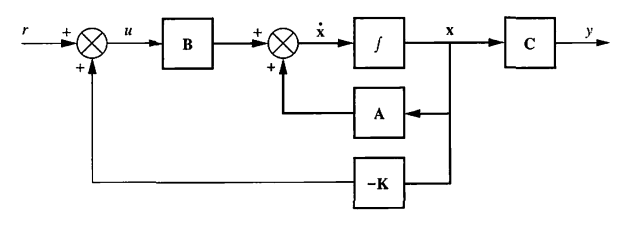
\includegraphics[width = 400pt]{Img/Controller_blok.png}
	\caption{Blok diagram over vores controller}
	\label{fig:Blok_CL}
\end{figure}

Vi gør brug af matlab funktionen place, som kan beregne vores state feedback matrix, K. Dette gør vi ved at indsætte state space variablerne A og B, som vi fandt frem til i starten og polerne fra vores karakteristik ligning. Dermed får vi beregnet vores feedback matrix så den passer med vores krav.
Nu kan vi teste om vores controller fungerer efter hensigten ved at smide et stepinput ind i systemet og kigge på responsen. Dette kan ses på \autoref{fig:StepOfSysSS_cl}.  

\begin{figure}[H]
	\centering
	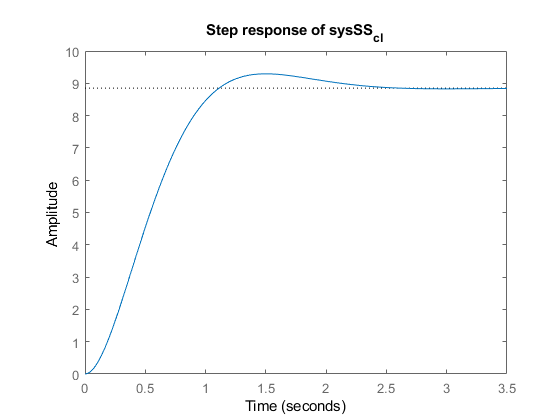
\includegraphics[width = 400pt]{Img/StepOfSysSS_cl.png}
	\caption{Steprespons for closed loop system}
	\label{fig:StepOfSysSS_cl}
\end{figure}



\subsection{Steady state error}

\begin{figure}[H]
	\centering
	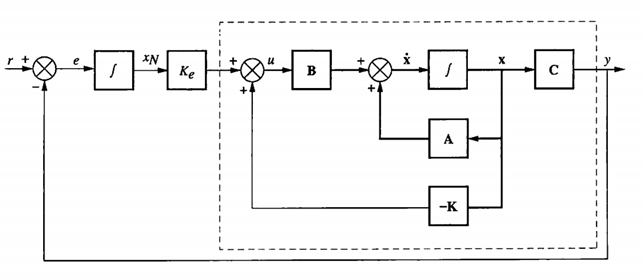
\includegraphics[width = 300pt]{Img/SteadyState_blok.png}
	\caption{Matrix når tredje pol indsættes}
	\label{fig:SteadyStateMatrix}
\end{figure}
For at fjerne steady state error skal en tredje pol indsættes


Man kan se på step responset at der er en stor steady state fejl. Denne fejl kan elimineres ved at indsætte endnu en pol i systemet. Denne pol skal gerne ligge så langt væk fra de eksisterende poler at det ikke har nogen indflydelse på systemets karakteristik. Til vores system vælger vi denne tredje pol til at ligge i -30. 

Da vi tilføjer endnu en pol og dermed også gør det til et tredje ordens system, bliver vi nødt til at lave om på vores state space matricer A, B, C og D. De skal udvides så de kommer til at se ud som på billedet nedenfor.

\begin{figure}[H]
	\centering
	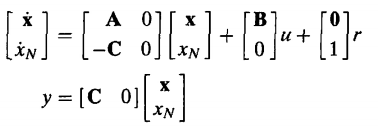
\includegraphics[width = 300pt]{Img/SteadyState_matrix.png}
	\caption{Matrix når tredje pol indsættes}
	\label{fig:SteadyStateMatrix}
\end{figure}

Denne matrix kan også laves på blokform. 
